\subsection{Grundkonzept des Benutzeroberflächen-Designs}
\label{subsec:grundkonzept-des-benutzeroberflachen-design}

In diesem Abschnitt soll das Grundkonzept der Benutzeroberfläche beschrieben und dargestellt werden.

Die Benutzeroberfläche wird in drei Seiten aufgeteilt, welche sich mit dem Einlesen der Daten, dem
darstellen und auswählen zu visualisierenden Daten und dem Ausgeben des Ergebnisses befasst.
Für das Navigieren zwischen den Seiten soll sich auf jeder Seite ein Navigationsmenü im oberen Bereich
der Seite befinden. Zudem sollen alle Seiten einen Bereich für Systemnachrichten wie Bestätigung oder
Fehlermeldungen und ein Label für die Seitenüberschrift besitzen.

Diese soll direkt unter dem Navigationsmenü angesiedelt werden, um die Grundstruktur identisch aufzubauen. In den nachfolgenden Text werden
die Konzepte der Benutzeroberflächen und ein grundlegendes Benutzungskonzept der einzelnen Seiten
anhand der Abbildungen \ref{fig: Benutzeroberflächenentwurf der Seite zum Einlesen der XML-Struktur},
\ref{fig: Benutzeroberflächenentwurf der Seite zum Ausgeben der Berichtstabelle} und \ref{fig: Benutzeroberflächenentwurf der Seite zum Ausgeben der Graphen} beschrieben.

Für das Einlesen der XML-Daten soll eine Eingabebox genutzt werden, in die die XML-Struktur kopiert wird.
Die Eingaben sollen über einen Button unter der Eingabebox bestätigt werden. Bei einem erfolgreichen
Einlesen und Einfügen in die Datenbank soll eine Bestätigungsnachricht im Bereich für
Systemnachrichten erscheinen. Bei einem Fehler soll in diesem Bereich eine Fehlermeldung mit
möglicher Lösung erscheinen. Der Aufbau dieser Seite ist in der Abbildung \ref{fig: Benutzeroberflächenentwurf der Seite zum Einlesen der XML-Struktur} dargestellt.

\begin{figure}[H]
    \centering
    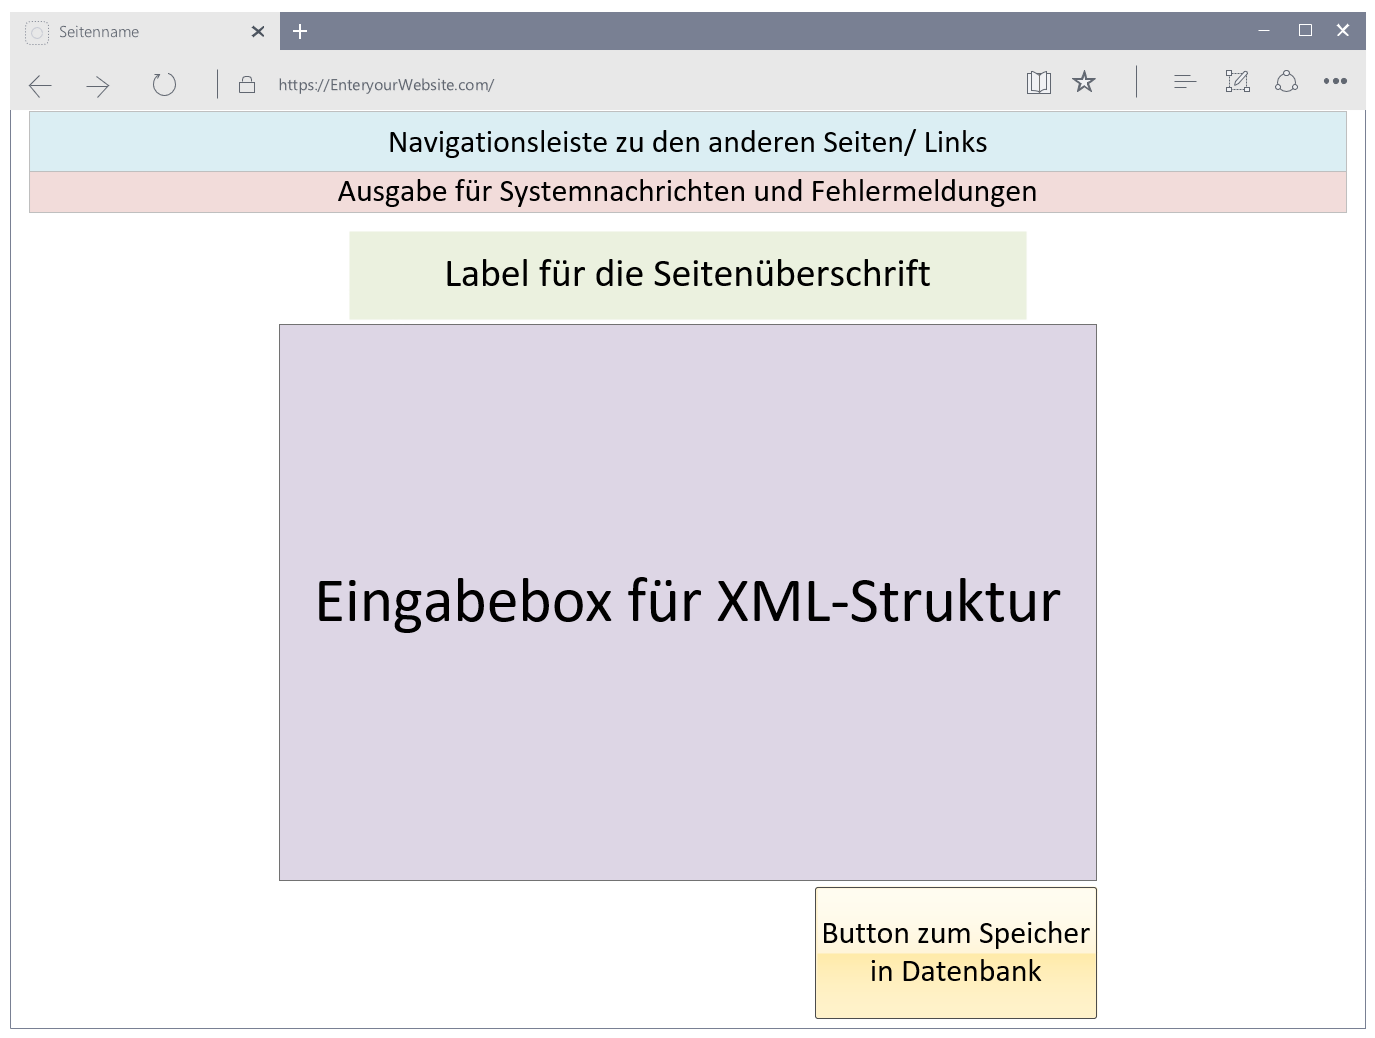
\includegraphics[width=0.95\textwidth]{Grafiken/Overlay_Einleseseite}
    \caption{Benutzeroberflächenentwurf der Seite zum Einlesen der XML-Struktur}
    \label{fig: Benutzeroberflächenentwurf der Seite zum Einlesen der XML-Struktur}
    {Quelle: Eigene Darstellung mit Microsoft Visio}
\end{figure}

Die Seite für das Darstellen und Auswählen der zu visualisierenden Daten soll im oberen Abschnitt der Seite
einen Bereich für Filtereinstellungen besitzen, mit möglichen Filteroptionen wie Datum oder Seriennummer.
Neben der Filtereinstellung sollen zwei Buttons für das Bestätigen und Zurücksetzen der Filtereinstellungen
sein. Bei einem Fehler bei den Filtereingaben soll im Bereich für Systemnachrichten eine Fehlermeldung
mit möglicher Lösung erscheinen.
Im unteren Bereich der Seite soll sich eine Tabelle, welche die eingelesenen Berichte in der Datenbank
anzeigt. Diese soll durch die Filtereinstellungen angepasst werden. Hierbei muss auf eine Anzeige
Möglichkeit für längere Tabellenstrukturen berücksichtigt werden, um die Benutzung effizient zu halten. Das
Das Grundkonzept ist in Abbildung \ref{fig: Benutzeroberflächenentwurf der Seite zum Ausgeben der Berichtstabelle} dargestellt.

\begin{figure}[H]
    \centering
    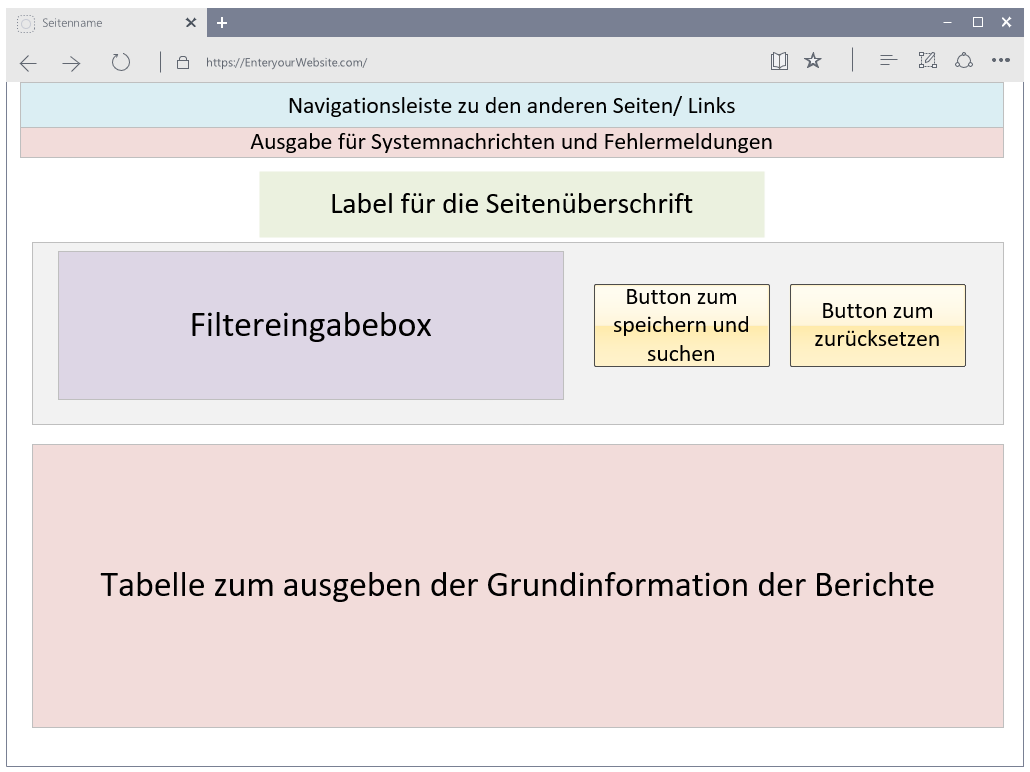
\includegraphics[width=0.95\textwidth]{Grafiken/Overlay_Tabellenseite}
    \caption{Benutzeroberflächenentwurf der Seite zum Ausgeben der Berichtstabelle}
    \label{fig: Benutzeroberflächenentwurf der Seite zum Ausgeben der Berichtstabelle}
    {Quelle: Eigene Darstellung mit Microsoft Visio}
\end{figure}

Für das Ausgeben der ausgewählten Berichtsdaten soll im oberen Abschnitt der Seite eine Instanz
eingefügt werden, die die Information zu den ausgewählten Berichtsdaten anzeigen.
Im unteren Bereich soll ein Label für die Seriennummer der ausgewählten Berichtsdaten eingefügt
werden.
Darunter werden die enthaltenen Module mit Labeln benannt, und unter diese Modulnamen werden
die Graphen und Werte für die visuelle Darstellung der Testdaten eingefügt. Die Anzahl der Darstellungen
hängt von den in den Bericht Daten enthaltenden Modulen ab. Die Anzahl und der Aufbau des Unteren
Bereiches ist variabel. Der grundlegende Aufbau dieser Seite ist in der Abbildung \ref{fig: Benutzeroberflächenentwurf der Seite zum Ausgeben der Graphen} dargestellt.

\begin{figure}[H]
    \centering
    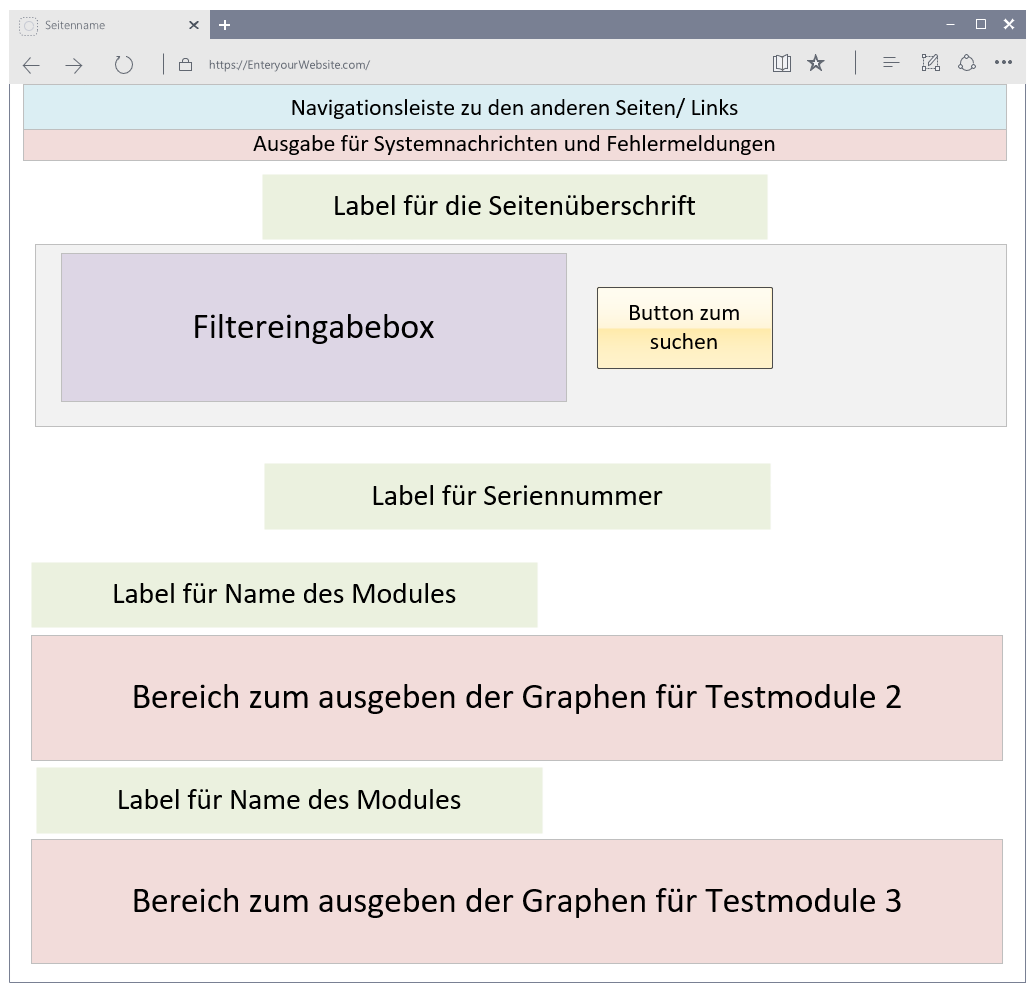
\includegraphics[width=0.95\textwidth]{Grafiken/Overlay_Ausgabeseite}
    \caption{Benutzeroberflächenentwurf der Seite zum Ausgeben der Graphen}
    \label{fig: Benutzeroberflächenentwurf der Seite zum Ausgeben der Graphen}
    {Quelle: Eigene Darstellung mit Microsoft Visio}
\end{figure}
















